\documentclass[12pt]{extarticle}
\usepackage{algorithm}


\usepackage{amsmath}
\usepackage{algpseudocode}
\usepackage[%
    left=1.3in,%
    right=1.3in,%
    top=1.1in,%
    bottom=1.1in,%
    paperheight=11in,%
    paperwidth=8.5in%
]{geometry}%

\usepackage[english]{babel}
\usepackage{blindtext}
\usepackage[]{hyperref}
\hypersetup{colorlinks=false,linkcolor=false,pdfborder = {0 0 0}
}
\geometry{top=2cm,bottom=2cm}
\usepackage{setspace}
\usepackage{graphicx}
\graphicspath{{images/}}
\onehalfspacing

\usepackage{pdfpages}
\usepackage{afterpage}

\usepackage[acronym]{glossaries}
\newacronym{ny}{NY}{New York}
\begin{document}
\newpage
\thispagestyle{empty}
{
\hypersetup{linkcolor=false}
\tableofcontents

}
\newpage
\pagebreak
\hspace{0pt}
\vfill
\begin{center}
\section{Introduction}
\end{center}
\vfill
\hspace{0pt}
\pagebreak

\subsection{Introduction}
These days, mobile robots have taken place in many fields like industry automation, planetary exploration, entertainment, and construction ..., for their ability to work in extreme environments with high precision and without fatigue\cite{rubio2019review}.Even so, a robot occasionally needs the support of other robots because it is impossible or difficult for them to perform some tasks on their own. For that, a new field has emmerged to deal with these problems, swarm robotics.

 
Swarm robotics is relatively a new research topic that has gained more attraction in the last few years. It is about  studying how a large number of simple robots (a swarm) can collaborate and work together to achieve predefined objectives and tasks that are often difficult or impossible to do for a single robot.\cite{bayindir2016review}.

One of the main challgenes that swarm robotics researchs face, is pattern formation. Where the agents (robots) try to form diffrent gemoetric shapes like squeres,trinagles and circles in order to perform a specific task.

We can solve this problem using two different aproches. The first one is a Centrelized method where there exist a centel unit  which controles the swarm and give global state access. However,  implementing this apporch  can be coslty and less robust to faillures. The second aproch is a dicentrilzed one, where each robot have uses local commucintion and have access only to his local state.\cite{bayindir2007review}

Our primary objective in this thesis is to implement an RL algorithm in a system made up of a group of robots in order to form some specific geometric patterns using a decentralized  method. Each robot will only have access to its local state and will interact and communicate with its neighbors in order to form the desired shapes.
 




\newpage
\pagebreak
\hspace{0pt}
\vfill
\begin{center}
\section{Swarm Robotics}
\end{center}
\vfill
\hspace{0pt}
\pagebreak




                  
\subsection{Swarm Intelligence and Social animal inspiration}
Social animal and insects behavior in groups like the bees dancing, wasp’s nest-building, ant's collaboration , bird flocking and fish schooling  has caught the attention of researchers for their ability to archive complex tasks and working in coordination, which demonstrate some form of swarm intelligence  that researchers have taken inspiration from to design and implement swarm robotics systems.\cite{navarro2013introduction} 

They also report that social insects were able to accomplish thier goals like searching for food, alerting the presence of an enemy, or collaborate to lift heavy objects, without having access to the global state or having a leader to guide them. They were only able to accomplish this by utilizing local interactions and communication, which spread to other members and and prompted group-wide cooperation.\cite{navarro2013introduction} 



\subsection{Swarm robotics and multi robot systems}
The early 1980s are when multi robots systems first gained popularity.
As the name suggests, multi robot systems introduce the idea of teamwork in order to complete tasks that are challenging or impossible to complete alone by the robots.
Seven topics of study have been identified in this feild which includes:
\begin{itemize}
  \item  Biological Inspirations; 
  \item Communication
  \item Localization, mapping, and exploration;
  \item Object transport and manipulation;
  \item Motion coordination; 
  \item Reconfigurable robots.
\end{itemize}
Swarm robotics is a subfield of multi-robot systems that differs from other multi-robot systems in some ways.\cite{arai2002advances}
   


 

\subsection{Swarm robotics}
Swarm robotics has no one definition because it is a rapidly developing area and new research is constantly being done in it. But we can take this defintion from a cited paper.
"swarm robotics is the study of how large number of relatively simple physically embodied agents can be
designed such that a desired collective behavior emerges from the local interactions among agents
and between the agents and the environment."\cite{csahin2005swarm}.\\

The main characters of swarm robotis are:
\begin{itemize}
  \item  The robots in the swarm must be autonomous. 
  \item The number of robots in the swarm is large.
  \item Homogeneity is required in robots. A small number is acceptable if not.
  \item Robots must be incompetent  with regard to the primary task they must complete, otherwise, they will fail or perform poorly.
  \item Robots are limited to local communication and sensing. It makes sure that coordination is spread, making scalability one of the system's characteristics.\cite{navarro2013introduction}
\end{itemize}


\subsection{Swarm robotics properties}
Swarm robotics have some properties that describe the system's current condition. Bellow are some of these properties:

\textbf{Robustness}: the ability of the swarm to  still function even with the loss of some members of the group or the faillure of some parts of the system.\\
\textbf{Scalability}: The ability of the system to perform well on smaller or larger group sizes without impacting the performance of the swarm.

\textbf{Flexibility} It is the capability of the swarm to adapt and manage the new changes that occur in the environment 

\textbf{Autonomus}: Implys that there is no central authority controlling the behavior of the swarm and each individual is independent of the others.

\textbf{Local communication} The communication among swarm members is local since they don't have access to  the swarm's overall state.
\cite{brambilla2013swarm}\cite{olaronke2020systematic} 

  

\subsection{Domain of application}
In this section, we will list some of the significant fields domains where swarm robotics fits in, and can impact in solving the domain problem.\newpage
\subsubsection{Tasks that cover a region}:
Because of the widespread sensing capabilities that the swarm has, swarm robotics is most suited for tackling problems that cover an area of the space, such monitoring the environment of a lake or  surveillance of a specific area.\cite{csahin2005swarm}\cite{olaronke2020systematic}

\subsubsection{Search and rescue missions}
In different types of accident or disasters that happen like earthquakes where the human intervention is difficult, swarm robots can be deployed for these type of missions. examples of such robots are: polyobot, swarm bot and M-TRAN.

\subsubsection{Cleaning of oil speals}
A swarm of robots can reduce the cost and time in such incidents. an exemple of robots that were deployed to such tasks is: Seaswarm, which was developed by the senseable group at MIT.

\subsubsection{Exploration}
To investigate Mars, swarm robots like Marsbees have been created. the same holds true for the CoCoRo swarm, which was employed for in-depth underwater investigation.
\subsubsection{Agriculture}
As they can be used to improve the agriculture and monitor the status of crops. 
\pagebreak
\subsection{Swarm robotics basic tasks and problems}
SR problems can be broken down into fundamental tasks that the swarm frequently carries out in an effort to accomplish its objective.
this tasks are: aggregation,d ispersion,pattern formation, coordinated
movement, hole avoidance and foraging\cite{bayindir2007review}\cite{navarro2013introduction}.

\subsubsection{Aggregation}
Aggregation of the robots is performed in order to accomplish some form or to exchange information. This problem can be easy in a centralized system, but  difficult in a decentralized one.
\subsubsection{Dispersion}
For exploration purposes, sometimes, the swarm must cover a wide range of area without losing the connection between the members, in order to expand the group sensing capabilities. 

\subsubsection{Pattern formation}
Sometimes, the swarm must form some specific patterns like circles,squares or  lines in order to lift some objects or traverse some ways corridors.
\subsubsection{Cordinated movement}
It is making an effort to coordinate the group movements by maintaining the established pattern between the robots.
\subsubsection{Hole avoidance}
As suggested by the name, the group makes an effort to avoid stepping into holes.
\subsubsection{Foraging}
The swarm aims to locate objects, pick them up, and position them where needed.

\newpage
\pagebreak
\hspace{0pt}
\vfill
\begin{center}
\section{Deep reinforcement learning}
\end{center}
\vfill
\hspace{0pt}

\pagebreak

\subsection{Introduction}
In this chapter we will provide an overview about the feild of reinforcement learning, including its applications, various techniques, and how it relates to swarm robots.\\
Before that,we will briefly discuss machine learning since it is the foundation of RL before we move on.
\subsection{Machine learning}
Machine learning is a sub field of artificial intelligence, which
focuses on developing algorithms and models that make prediction and take decisions without being explicitly programmed to do so
based on the input data they receive.
Generally speaking, there are three types of machine learning algorithms,
suppervised algorithms which obtain labeled data and attempt to categorize or anticipate the unknown one. Unsupervised learning algorithms, where the  data is unlabeled and it is the job of the ml algorithms  to extract  hidden patterns in it. And finally, reinforcement learning algorithms  where the algorithm learns to make decisions based on trial and error and rewards, by interacting with an environment.

\subsection{Reinforcement learning}
Reinforcement learning algorithms are based on a agent that interact and observe  an environment in order to take actions that maximize the reward for a given task.

The goal of the agent is to learn an optimal policy ($\Pi$) which maps state to actions in order to get the best possible action to take in a given situation. This can be achieved  by maximizing the expected  reward that the agent receive from the environment on each step he takes.\cite{arulkumaran2017brief}

Formally, RL can be described as a Markov Decision Process (MPD) where the future state depends only on the current one. An MPD  consists of:

\begin{itemize}
  \item  A set of states $S$
  \item  A set of actions $A$
  \item  A transition dynamics $\rho(S_{t+1}|a,S)$. which give the probability of being in state $S_{t+1}$ based on the current state $S$ and the performed action $A$.
  \item A reward function $R(S_{t},A_{t},S_{t+1})$ which outputs a scalar reward $r_{t} \subset R$. 
   \item A discount factor $\gamma \in [0,1]$ which  emphasis either  immediate or future rewards.
\end{itemize}

\newpage
From the above definition, the policy function $\Pi$ will  a map a given state to a probabilty distribution over actions: $\Pi: S \longrightarrow \rho(A=a|S)$.
The goal of the agent to find the optimal policy $\Pi$ which maximize the expected return :\\
\[ \Pi^{*} = argmax_{\Pi}  E[R|\pi] \]

If the MPD is episodic, then the agent will accumulates a set of reward at the end of each episode which is called a return:

\[ R= \sum_{t=0}^{T-1} \gamma^{t}r_{t+1} \]

Setting $\gamma<1$ will ensure the convergence of the return in case of non episodic MPDS.\cite{arulkumaran2017brief}.

\subsection{Q learning}
Q-learning is a type of model free reinforcement learning algorithm  based on the dynamic programming technique, where the agent tries to maximize it rewards by finding the optimale policy $\Pi$ in an iterative manner. In order to  acheive this, the agent uses a type of equation called value function that gives it the value or the reward of being in a state $s$ and taking action according to it policy $\Pi$.


\[ V^{\Pi}(S)=E[r(s,a)+\gamma V^{\Pi}(s') ] \] 

In order to find the optimal value function, hence finding the optimal policy, the equation must satisty the bellman optimality condition which states that: 

  
\[ V^{*}(S)=max_{a}E[r(s,a)+\gamma V^{*}(s') ] \] 

The same goes for the action-value function which gives the return if the agent chooses the action $a$ and follow the optimale policy thereafter.

\[ Q^{*}(S,a)=E[r(s,a)+max_{a}\gamma Q^{*}(s',a) ] \]\cite{watkins1992q}.


\pagebreak

\subsection{Deep Q learning}
The problem with traditional Q-learning or Rl algorithms in general, is the inability to work in  a high dimensional input states where discritization and hand-crafted features extraction    is performed in order to it to work. For this, deep learning was combined with traditional Q-learning in order to overcome these challenges.\cite{mnih2013playing}

Deep Q learning was firstly introduced in an article by the deepmind group, where it was tested in atari games in which the agent was given raw input images of the emulator and it was the  goal of the agents to win the games by using the Q learning algorithm.

Besides using the bellmen equation to converge and calculate the loss, an experience replay memory was used to store the the experiences of the agents during  the game and then sampled randomly to be  fed to the neural network to learn and in order to break the correlation that apears when fedding them sequential data.\cite{mnih2013playing}
 
\begin{algorithm}
\caption{Deep Q-learning with Experience Replay}\label{alg:cap}
\begin{algorithmic}
\State Initialize replay memory D to capacity N
\State Initialize action-value function Q with random weights
\For{\texttt{episode = 1, M}}
        \State \texttt{Initialise sequence s1 = \{x1\} and preprocessed sequenced $\phi_{1}$ = $\phi(s_{1})$  }
        \For{\texttt{t = 1, T}}
         \State With probability $\epsilon$ select a random action $a_{t}$
         \State otherwise select  $a_{t}$ = $max_{a} Q^{*}(\phi(s_{t},a;\theta) $ 
         \State Execute action $a_{t}$ in emulator and observe reward ${r_{t}}$ and image $x_{t+1}$
        \State Set $s_{t+1}$ = $s_{t}$ , $a_{t}$ , $x_{t+1}$ and preprocess  
        $\phi_{t+1}=\phi(s_{t+1})$
        \State Store transition $(\phi_{t} , a_{t} , r_{t} , \phi_{t+1} )$ in $D$
        \State Sample random
minibatch of transitions $(\phi_{t} , a_{t} , r_{t} , \phi_{t+1} )$ in $D$
        \State set  \begin{equation}
  y_{j}=\begin{cases}
    r_{j}, & \text{for terminal $\phi_{j+1} $}.\\
    r_{j}+\gamma max_{a}Q(\phi_{j+1},a';\theta) , & \text{for non-terminal $Q(\phi_{j+1})$}.
  \end{cases}
\end{equation}
        \State Perform a gradient descent step on $(y_{j} - Q(\phi_{j} , a_{j} ; \theta))$ 
        \EndFor 
\EndFor 


\end{algorithmic}
\end{algorithm}
 


\pagebreak

\subsection{Deep Deterministic policy gradient }
One of the major problems of DQN is that he works only in discreate action spaces. For this, tasks that require continuous control, such as the linear and rotational movements of robots, require discretization. In most cases, this can result in a large action space, which slows convergence and causes instability.. \cite{lillicrap2015continuous}

For this, there is another type of DRL algothims named Deep Determinisitc policy gradient, which is a policy based method actor critic algoithm, that takes the benifites of both methods (policy based method and value based method, and useses the actor critic to reduce the bias (underfitting) that occurs ...

DDPG in  composed  of two neural networks: the actor and the critic. The job of the actor is to select an action based on the input state. And it is the critic who will determine if that action was suitable or not by observing the rewards  returned when taking that specific action in a specific state.

The critic network is  learned using bellman equation same as q-learning.

The DDPG algothim also useses a replay buffer to store agent exepriences
in order to sample from them later when training the netwroks.

Like in Q-learning and to enable better exploration for the agent, a noise 
is sampled from a process $\eta$  then added to the output of the actor network. It is common to use the Ornstein-Uhlenbeck process to generate temporally correlated values.\cite{lillicrap2015continuous}





 
\begin{algorithm}[H]
\caption{Deep Deterministic Policy Gradient (DDPG)}
\label{alg:ddpg}
\begin{algorithmic}[1]
\State Initialize actor network $\mu(s|\theta^\mu)$ and critic network $Q(s,a|\theta^Q)$ with weights $\theta^\mu$ and $\theta^Q$
\State Initialize target networks $\mu'(s|\theta^{\mu'}) \leftarrow \mu(s|\theta^\mu)$ and $Q'(s,a|\theta^{Q'}) \leftarrow Q(s,a|\theta^Q)$ with weights $\theta^{\mu'} \leftarrow \theta^\mu$ and $\theta^{Q'} \leftarrow \theta^Q$
\State Initialize replay buffer $R$
\For{episode $=1$ to $M$}
\State Initialize a random process for action exploration
\State Receive initial observation state $s_1$
\For{$t = 1$ to $T$}
\State Select action $a_t = \mu(s_t|\theta^\mu) + \mathcal{N}t$ according to current policy and exploration noise $\mathcal{N}t$
\State Execute action $a_t$ and observe reward $r_t$ and new state $s{t+1}$
\State Store transition $(s_t, a_t, r_t, s{t+1})$ in $R$
\State Sample a random minibatch of $N$ transitions $(s_i, a_i, r_i, s_{i+1})$ from $R$
\State Set $y_i = r_i + \gamma Q'(s_{i+1},\mu'(s_{i+1}|\theta^{\mu'})|\theta^{Q'})$
\State Update critic by minimizing the loss: $\mathcal{L} = \frac{1}{N}\sum_i(y_i - Q(s_i,a_i|\theta^Q))^2$
\State Update actor policy using the sampled policy gradient: $\nabla_{\theta^\mu} J \approx \frac{1}{N}\sum_i \nabla_a Q(s,a|\theta^Q)|{s=s_i,a=\mu(s_i)} \nabla{\theta^\mu} \mu(s|\theta^\mu)|_{s_i}$
\State Update target networks: $\theta^{\mu'} \leftarrow \tau \theta^\mu + (1-\tau)\theta^{\mu'}$ and $\theta^{Q'} \leftarrow \tau \theta^Q + (1-\tau)\theta^{Q'}$
\EndFor
\EndFor
\end{algorithmic}
\end{algorithm}

\subsection{Related Work}
In this section, we present some of the work that have applied RL algorithms in  training agents and robotics systems.


The most used algorithm  is Deep Q learning, where  \cite{mnih2013playing} have applied it in learning playing atari games by using a convolutionnal neural netwrok by providing raw image pixels as input, where they demonstarted that the agents achived great performance even surpassing human level.

In continous action spaces, \cite{lillicrap2015continuous} have used the ddpg algorithm, which is an extension of the DQN and the DPG algorithms. They have used an actor critic model free  policy based algorithm which operate in conitous action space by appliyng it in several simulated physics tasks, and also shows great result achived by the agents.

In field of multi agents. \cite{diallo2020multi} where they used a decentrilized aproach to train multi agent to form some patterns using the DQN network with  a central replay buffer that contains agents experinces in order for them to learn cooparitvly.


For robotics, \cite{long2018towards} have used the Proxiaml policy optimization algorithm (PPO) wchih is a policy based one , to controll in a decentrilzed manner a group of robot to reach their target by avoidng collison between them. Also in \cite{ma2020multi} have used the ddpg algorithm to traing mutli robtos to encircle some target in a static position  or in mouvement where the agents (robots) learn to coopretivly achevce their task by using also a central replay memory.
 

Finnaly, in \cite{dong2020mobile},\cite{gong2022efficient} and \cite{quiroga2022position} have applied the ddpg and dqn algorithms for path playing and postion control of robots in order to achive the target goals.






 

  
  
  
\newpage
\pagebreak
\hspace{0pt}
\vfill
\begin{center}
\section{Problem formulation And Solution Conception}
\end{center}
\vfill
\hspace{0pt}

\pagebreak

 

\subsection{Introduction}
 In this section, we'll go into  detail about the objective that needs to be accomplished by our robots, the difficulties they must overcome, and then our suggested solution.
 
\subsection{Goal defintion}
Our objective in this thesis is to make multi robots  form geometric patterns like lines, circles, squares, and triangles while avoiding collisions and moving toward their destination in a quick and efficient manner. 



\subsection{Problem Formulation}
 

\subsubsection{Environement}

We will describe our multi robot environemnt as an MDP where $S$ are the set of states that each robot will reacive. $A$ are the set of actions that it can take , and $R$ are the set of rewards that each robot will get during each episode. The  goal of each robot is to  maximize his return by reaching the goal target and avoiding collisons with the wall and other  robots. We will use the DDPG alrorithm to controll the robots in a contious manner.




For the environemnt, we will Consider a scenario in which there are n ($n >  2$) robots moving in a 2D environment. Each robot will try to reach his target position which is descibed by the homogeneous coordinates (x,y)  that is be set by the  central robot.


 
 \begin{figure}[h]  
\centering
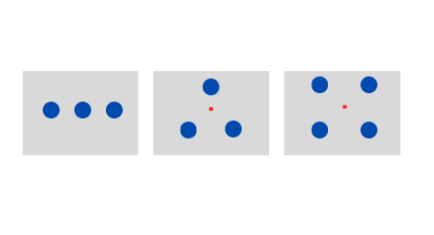
\includegraphics[scale=0.4]{formation}
\caption[formation]{formation}
\end{figure}

\pagebreak
\subsubsection{Shape generation}
In order to form the different shapes, The central or leader robot will first go to a point in the space and from it , he will inform  other robot with the desired shape to be formed by giving them their target position relative to his position by being at a certain distance and angle.



\subsubsection{Shape formation Algorithm}


\begin{algorithm}[H]
\caption{Shape Formation Algorithm}
\label{alg:ddpg}
\begin{algorithmic}[1]

\State Initialize $n=N$ number of robots.
\State Initialize $c=0$ goal counter.
\State Assign each robot an id starting from $id=1...N$

\State Set the central robot with $id=1$.
\State The central robot  chooses a random postion and stay on it.

\State The central robot broadcasts a message containing his position with the desired shape by using generaing a set of cooardinates that each robot must reach.
\While{$c!=N$}
\For{robot in robots}
\State Take an action.
\State Inform the central robot with his current postions every $t seconds$.
\If{target position reached} 
    \State Stop the robot and inform the central robot.
    \State $c++$ 

\EndIf 

\EndFor

\EndWhile

\end{algorithmic}
\end{algorithm}

\subsubsection{Explanation}

The first robot will choose a random position and place himself in it. Then he broadcast a message containing his position and the target positions to other robots in order to form the shape by using the distance and the angle.

Once the message is received by other robots, each one of them will try to reach the target goal autonomously by avoiding collision with other robots.
And once they reach their goal they will inform the central robot with their task completion.

Finally, and if all robots are in place, the central robot will check  the state of the formation and declare the task  as complete if  the shape is formed correctly .







\subsection{State Representationn}

\subsubsection{Introduction}
The state and reward function must be well designed in order to generate the desired shape because how they are represented will directly impact our robot's performance towards achieving their goals and the architecture of the neural network.


\subsubsection{State Representation}
The state of the robots will be  the inputs for our neural networks and  based on them, we can  calulate  the rewards that the robot will get when acting in the environement.

In our implementation we have defined six kind  of state information, the distance to goal, angle to goal, angular velocity,linear velocity ,the minimun detected object distance and it's angle for collision avoidance.




\begin{itemize}
\item \textbf{The distance to goal}: 
The first component in our state representation is the distance to goal, which will be calculated using the euclidean distance  between the robot and the goal .


\[ D(P,G)=\sqrt{(Py-Gy)^2+(Px-Gx)^2}  \] 

Where P and G are the current homogeneous coordinates of the robot and the target goal respectively.

\item \textbf{The angle to goal}: 
The second component  is the angle  to goal. And to find it we need to calculate  the difference between the robot yaw, which is it's orientation around it's vertical axis, and the angle between the goal and the robot positions.


\[ \theta(P,G)=yaw-arctan(P/G)  \] 


\item \textbf{The minimum detected distance}: 
In order to detect other robots and avoid collision, we use an  LDS   which gives us an array of elements where each value is the minimum distance detected and each index is the angle of detection.


\item \textbf{The angle of detection}: 
It is is the angle of the detected object relative to the robot lds.

\item \textbf{The angular veloctiy}: 
It is the angular or rotational mouvement of the robot, and it's between 
$ -\Pi $ and $\Pi$.

\item \textbf{The linear veloctiy}: 
it  is the linear speed of the robot . and we have set it between 0.2 and 0.5 m/s.

\end{itemize}

These information will help the robot to make decesion when expoloring the environemnt and each one of them has it's importance and purpuse.






\subsection{Reward Function Design}

The reward function design is a critical part of any RL system. A well designed reward function will give the  robot more feedback when acting in the environment thus making the task more straight forward.

The reward function was designed to engourge and reward the robot  more, when he  aproches the goal target, and penilize him when he collide with the wall or other robots.

The design of the function is based on the state. We have used the distance , the  angle and the LDS to form the final function.

We have   divided  the function into three parts:
The first part is  the distance reward. We will give the robot more reward when he aporoches the target goal and less when he doesn't:
   
\setcounter{equation}{0}

       \begin{equation} \label{dist_r}
     R_{D}=-D_{goal}
   \end{equation}
 Where $D_{goal}$  is the changing distance between the robot and the target goal,
    
The second part is to the angle of the robot to the goal. formally:



     \begin{equation} \label{angle_r}
     R_{\theta}=-\theta_{goal}
   \end{equation}
 
 where $\theta_{goal}$  ranges  between $-\pi$  and $\pi$.
  
And For avoiding collion between the robots and the wall, we have set two values. The first one is set  when the robot aproches the object which can lead to a collision. And the second one is when is actualy collide  with it.


\begin{equation}  \label{obs_r}
  R_{c}=\begin{cases}
    -10, & \text{if $mdd< 0.6m$}.\\
    -500 , & \text{ if $mdd <0.13m$ (a crash )}.\\
    0 & \text{ else}.
  \end{cases}
\end{equation}
where $mdd$ stands for the minimum detected distance.\linebreak
Finally, we can add \ref{dist_r}, \ref{angle_r} and \ref{obs_r} to form the finale reward function: 

 
    \begin{equation} \label{final_r}
     R=R_{D}+R_{\theta}+R{c}
   \end{equation}






\pagebreak



\subsection{Formation and Deep Reinfocement Learing}
\subsubsection{Introduction}


Each robot will have it's own neural network which will guide him towards the goal positions by avoiding collision with other robots.

As  mentioned earlier, we have used the DDPG algothim where each robot will have two neural networks, the critic and the actor.

The actor model will get as input the mentioned state and outputs two actions: the angle and the velocity.

The robot will learn to  move towards the goal by adjusting the angle and will use the velocity to learn how to move faster in certain conditions and when not. For example the velocity will
help him in colision avoidance. If he doesn't detect any robots in front of him  he moves faster, else he slows down.


For the critic, he gets as input both the state and the actions, and outputs the q-value which will be used by the actor to choose the suitable actions to take.

The parameters of both networks will affect how the performance of the robots and the speed of convergence. we will describe in details the parameters that we have chosen to be good for achieving the task.

\subsubsection{The learning flow}
Here, we will describe the learning flow that the robots will go through to learn how to aproach their goals.

It starts by the robot being in a given state, he then takes an action,  reacive sensor data from the sensors like lds and imu, then based on them we calculate the reward function and finaly the robot transition to a new state.

This information (state,action,reward,next state) will be stored in a replay buffer to sample from it during the training of the models , and once he reaches a certain number of experiences the training starts.



If all robots reach their goal, the simulation is reset and a another formation shape is generated in order to prevent overfitting a certain type of shapes.

And if they collide the simulation is reset also and the robots tries again to form the desired shape.

This learning flow will continue until the models converge and the robots form the shapes many times respectively.


 \begin{figure}[h]  
\centering
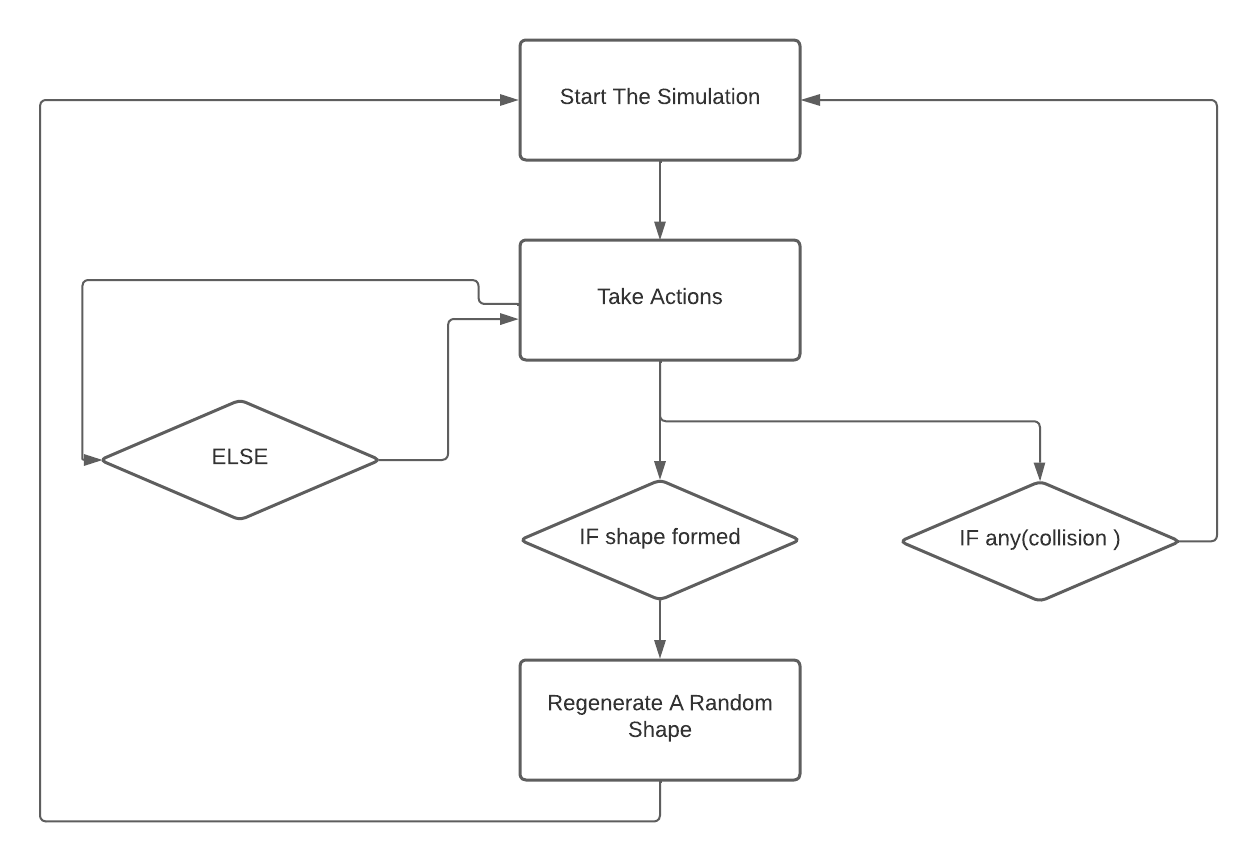
\includegraphics[scale=0.85]{simulation_flow}
\caption[simulation flow]{simulation low}
\end{figure}







 \begin{figure}[h!]  
\centering
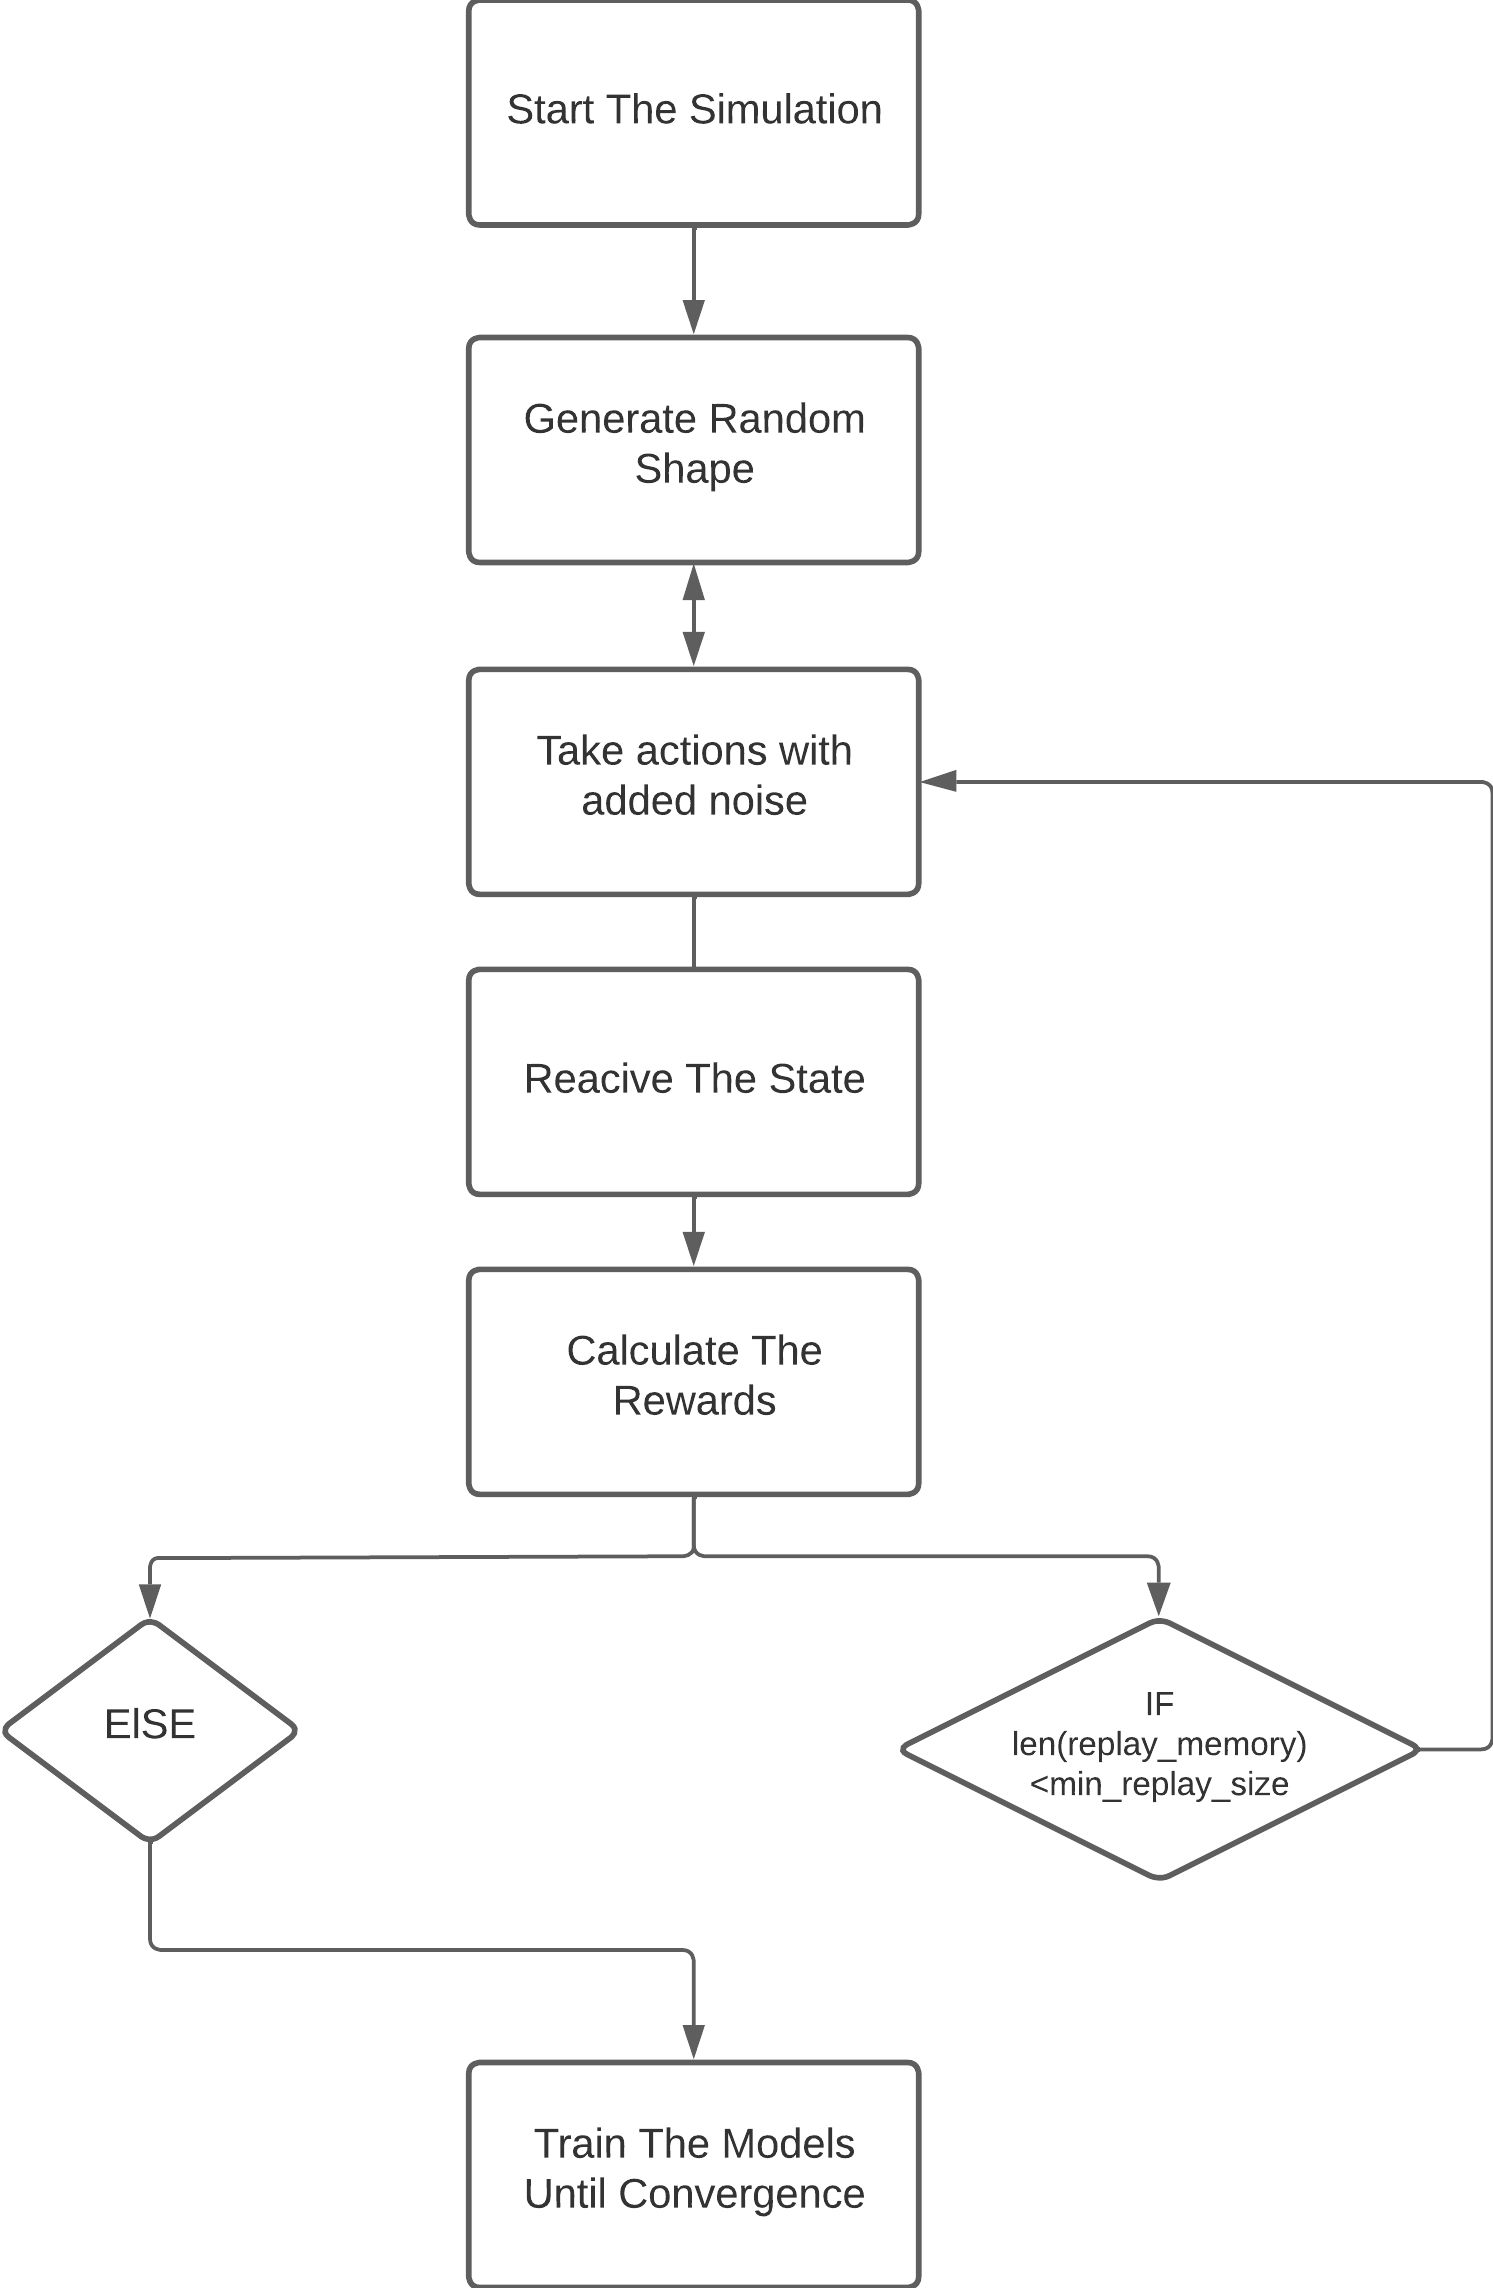
\includegraphics[scale=1]{training_workflow3}
\caption[training flow]{training flow}
\end{figure}


\afterpage{\clearpage}

\newpage
\pagebreak
\hspace{0pt}
\vfill
\begin{center}
\section{Implementation}
\end{center}
\vfill
\hspace{0pt}

\pagebreak




\subsection{Introduction}
In this section, we will explain how we have implemented the solution , how the neural networks are designed, what frameworks, tools and simulators used to train and test the robots shape formation. 












\subsection{Roboting Operating system}
To implement our work and test it, we used the roboting operating system (ROS), which is  a collection of open source software and tools, that 
 simplifies our work by giving us the necessary tools for controlling the robots, determining their positions and angles, gathering sensor data and preparing it for manipulation, and also giving the robots a way to communicate with one another.

\subsubsection{Ros Basics}
There are five concepts that ROS is built on that will allow us to implement our solution in  simple and modular way.


 

\begin{itemize}
\item \textbf{Nodes}: Ros is made up of nodes where  each node     is responsible for a single giving task like moving the robot, getting sensor data, doing some processing ... 
nodes can communicate between each other using topics and services.

Each node can subscribe or publish  to one or more topics. he can contains also one or more services which other nodes can request to get a one time information. This approach used by ros will allow for modularity and more organized and clean code.

     



\item \textbf{Topics}: ttopics are a way for nodes to communicate between them. Each node can either subscribe to a topic thus reaciving informations from other nodes, or publish to some topic to send information to other nodes.

For example: a node can subscribe to a topic that publish the position of the robot  from another node which is responsible for providing this information.

When defining the topics, we first need to define the exact type of information that they will receive. For instance, we can define topics to accept only string ,numbers, arrays or we can define our custom data type..


\item \textbf{Services}:  They are the same as topics but they differ in that data is received when requested by a client in contrast to topics where there are a stream of data updated continuously. This can be helpful in situations where the inforamtion is needed only once or the update frequency of it is low.
 


For example: We can have a service that generate goals or reset the simulation.

Same as topics, we  must set the data type that the services work with.


\end{itemize}
 

 
 \begin{figure}[h]  
\centering
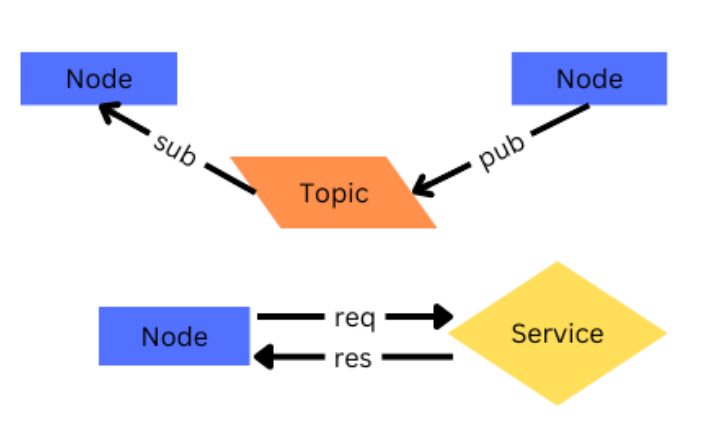
\includegraphics[scale=0.4]{ros}
\caption[Ros]{Ros}
\end{figure}


Ros support  c,c++ or python as programming languages. in our project, we choosed python. 
For the operating system, Ros support mainly linux systems, the support for windows was added until recently. We have used ubuntu for the existing support and large ros community .







\subsection{TurtleBot}
We will be using the turtlebot robot which is developed by open robotics. The same organization behind ros and the gazebo simulator.

This robot is used for educational,research and prototyping purposes, where multiple version have been developed. In this thesis, we will be using the turblebot3-burger version.\cite{turtlebot}

\subsubsection{TurtleBot3 components}
TurtleBot3 is a two wheeled, small  size  lightweight  robot  equipped with a variety of sensors, including a 360-degree laser rangefinder for obstacle avoidance, and an IMU for navigation and localization. The robot is powered by a Raspberry Pi single-board computer and it is compatible with ROS.
 \begin{figure}[h]  
\centering
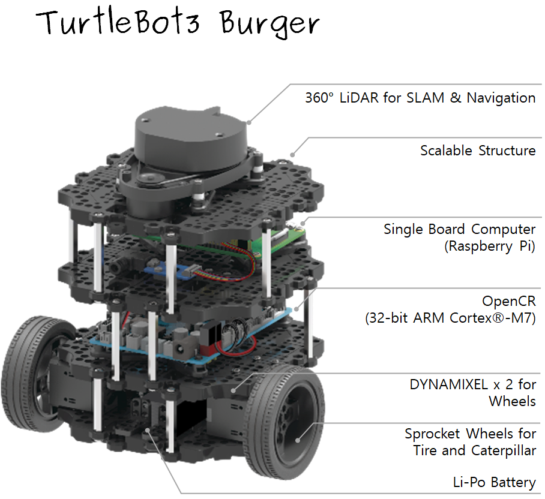
\includegraphics[scale=0.4]{turtlebot3_burger_components.png}
\caption[TurtleBot3]{TurtleBot3 [\textbf{ref}:https://emanual.robotis.com/]]}
\end{figure}

\begin{itemize}
\item \textbf{LDS}:  LDS, which stands for laser distance sensor. which uses laser to detect the distance between the robot and it's surrounding to allow the robot to navigate in the environment and avoid detected obstacles. The used LDS in this project can  sense object in 360 degree with a maximum length of 3.5 meters.
 
The (LDS) was one of the data  source to train our neural networks besides the robots positions. we have used it to detect other robots and to avoid collisions during the navigation. we have minimized the original 360 sample from the LDS as no need for such precision in our project. 

     
\item \textbf{IMU}: IMU stands for Inertial Measurement Unit, is a type of electronic sensor that is used to measure the orientation, position, and velocity of a moving object. The IMU combines information from many sensors, such as accelerometers, gyroscopes, and magnetometers, to give a thorough picture of the movement of the object in three dimensions. The position of the robot is calculated relative to a fixed  reference frame which either define by the system designer like a closed room or factory or by the robot himself in outdoor environment.







\end{itemize}

   



\subsection{Simulation}
It's hard , time consuming and  costly to train the robots in real world. For that, simulation is used to train the robots as it allow us to train in a faster repeatable way,  let us put the robots and the environment  in different conditions  for faster experimentation.


Robotics simulation programs like Gazebo, Webots, V-REP, MATLAB Robotics System Toolbox, and CoppeliaSim are some of the more well-liked ones. each one of them has it's own features from programming language support to cost fee.

In our project we used the gazebo simulator as it is free, open source and integrate well with Ros.

Gazebo is an open source collection of software libraries that have been developed for robotics developers and educationist.

It allows  to simulate  robotic systems in a virtual environment, providing a safe and cost-effective way to test and refine robot designs before deploying them in the real world. It contains a lot of prebuild models sensors and give the user the ability to build custom ones. Gazebo is also able to simulate real world physical phenomena, including physics-based motion, collision detection, and sensor simulation.

  
 \begin{figure}[h]  
\centering
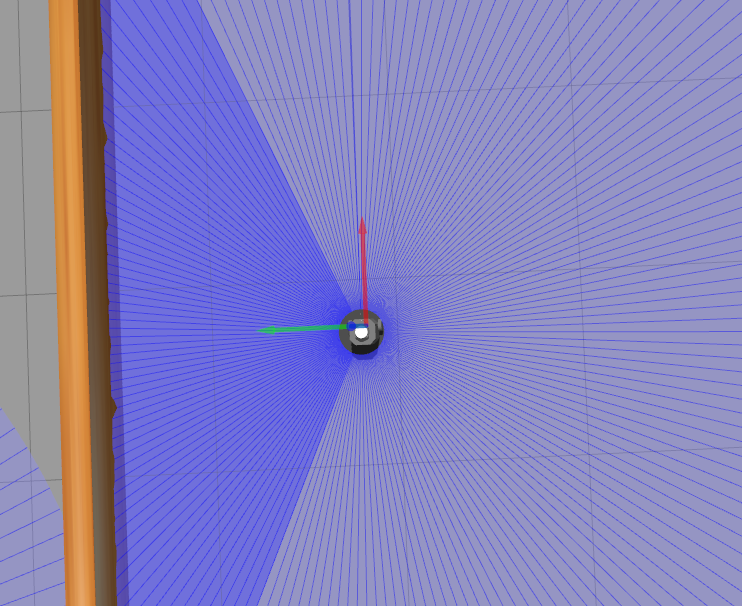
\includegraphics[scale=0.4]{lds.png}
\caption[Lds]{TurbleBot3 Lds}
\end{figure}






 
   











 

\subsection{Ros implemation}
In this section, we will describe how we have implemented our solution in ros, how we defined the different nodes, topics and services that makes up the system.

The work is divided into phases. The first phase is the training and test phase and the second one is the deployment phase.

In the first phase we implemented the solution in ros in a way to facilitate the training process that will require a lot of modification of code and simulation replay. In this phase   we haven't set the networking between the robot as we assume that each robot knows his target positions and we assume that we can access the global state.  as this is will l....


For the second phase, and after the models are trained we will deploy them in each robot and each robot will choose his actions based on his model, and also will communicate with the central robot for coordination.


\subsection{Ros implemation: Training phase}

We have followed the openai gym implementation of  rl problems using the python programming language.

In the training phase, we have defined two nodes and one python class for the neural networks.
 

The first node is the environment node. This node is responsible for getting sensor data, positions and command robots to move in the simulation.

This node have one service, subscribe to  two topics and publish to one. The first topic he subscribe to is the Laser topic which gets the laser measurements of each robot every step. the data returned   by this topic is an array where each element of it contains the distance of the detected object and the index of this element is the angle of detection.


The second topic he subscribes to is the positions topic, which will get the x,y coordinates of the robots and also their orientation. For the topic, the node will publish to it instead of subscribing. he will publish the actions that the robot must take based on the output of the neural network.

The service that this node offer for the main node is  a function that will take that actions that the robots should take , get the states,calculates the rewards and then passing back the response to the main node. 

This node is also responsible for calculating the rewards based on the state.

We called the second node the main node. This node is responsible of starting the main training loop,getting actions from the models passing them to the environment node in order to reactive the next states and the rewards, he then store these samples in the replay memory and finally train the models.
The loop will continue until the models converge and the shapes are been formed. This node will connect to a python class which contains our models.


This python class defines the models and the networks architecture, contains the replay memory and describes the training process.  

 \begin{figure}[h]  
\centering
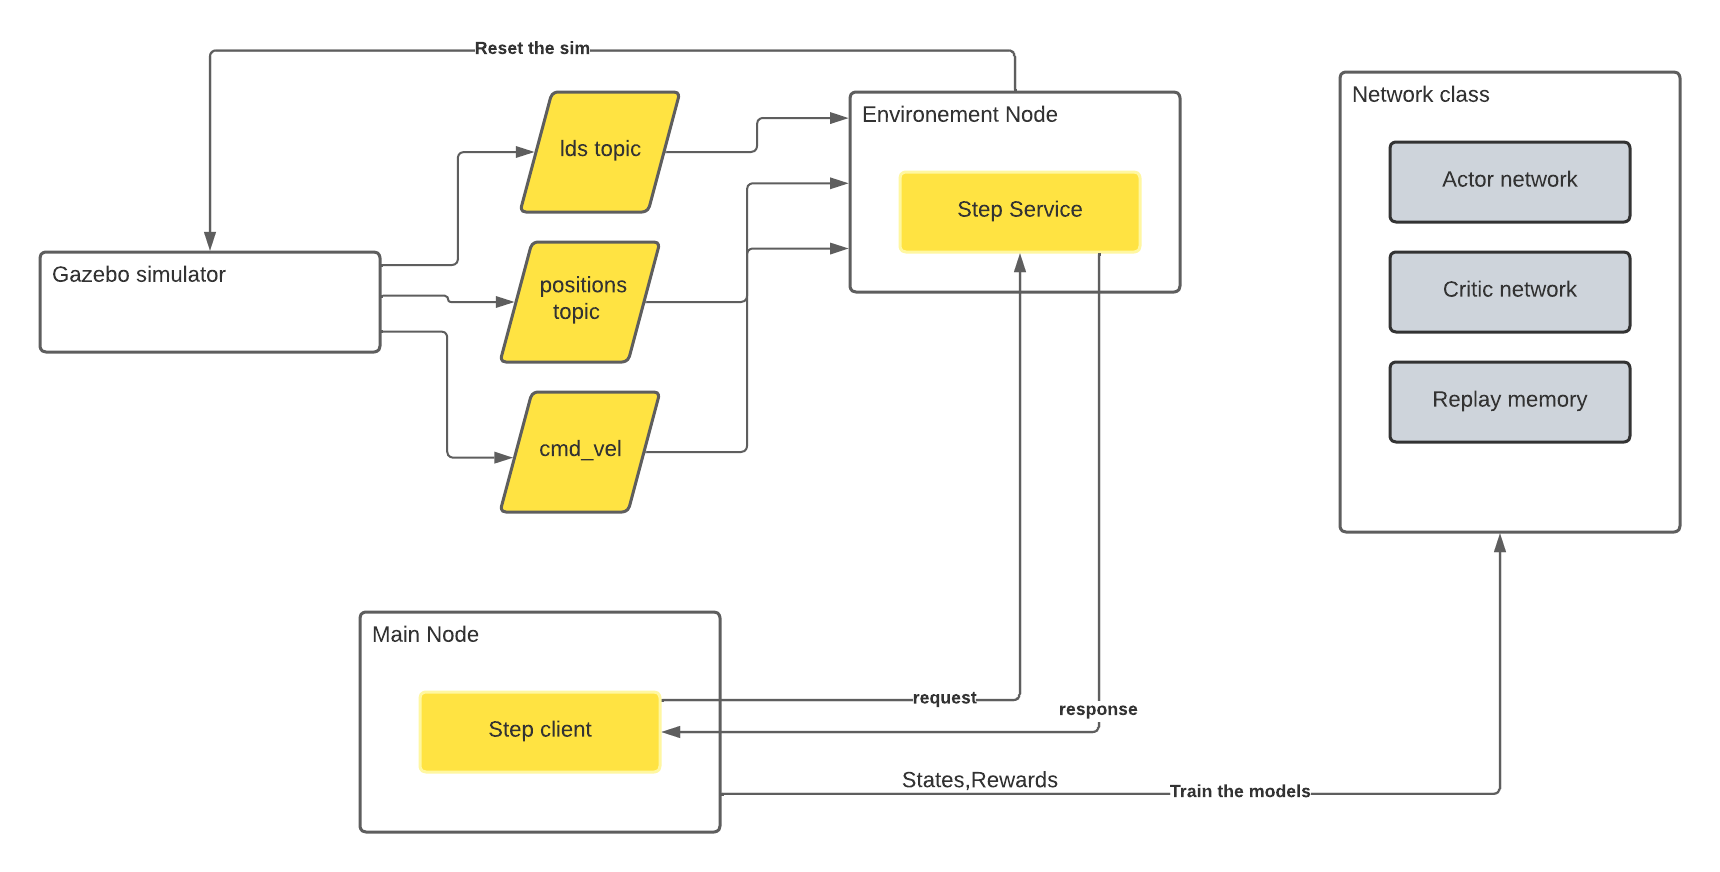
\includegraphics[scale=0.6]{training}
\caption[training phase]{training}
\end{figure}

\pagebreak

\subsection{Ros implemation: Test phase}
In this phase, and after the training of the models is done, we will deploy  just the actor models on each robot (no need for the critic as no training is happening)  in order to him to take actions based on the input state.

We have set a node for each robot, therefore the communication will take place  between this nodes by defining custom topics. Each node will get input state and pass them to the actor network to predict the actions to take.

We have defined one topic called the goals topic in which the central robot will publish the goal positions and the others subscribe to it. We have also defined a service in the central robot that the others 




 \begin{figure}[h!]  
\centering
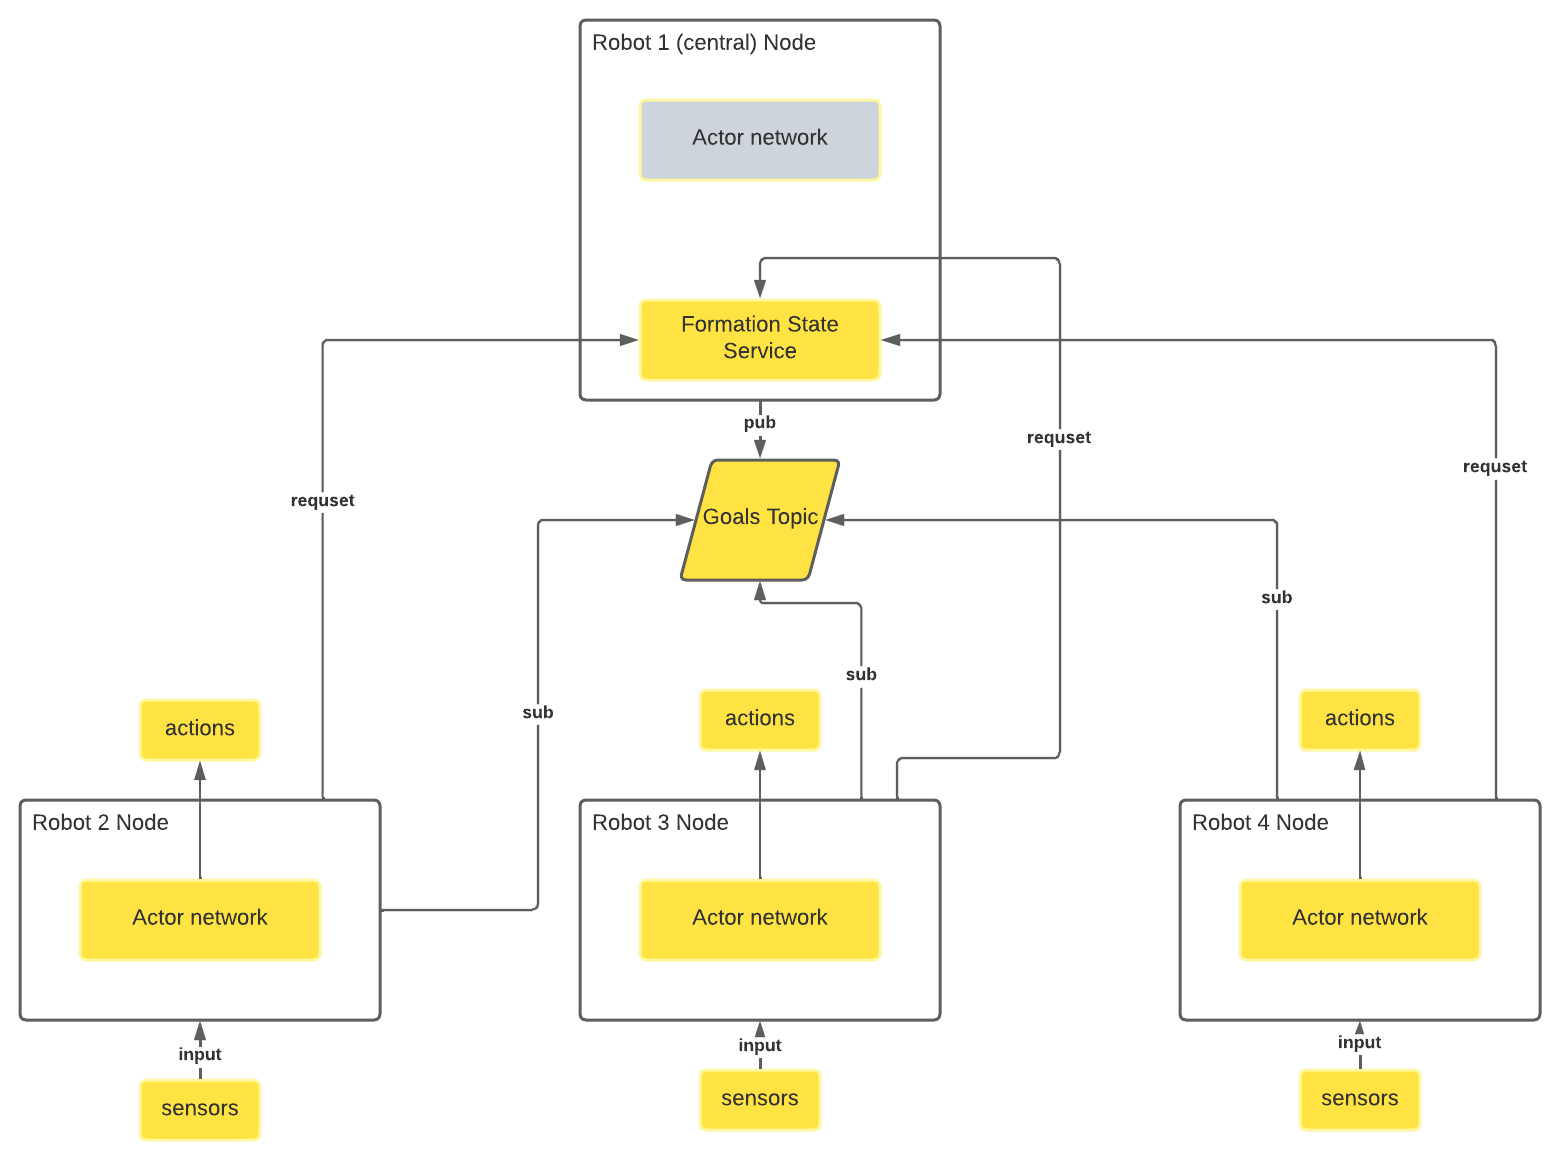
\includegraphics[scale=1]{deployment}
\caption[deployment]{deployment}
\end{figure}










 
\newpage




\subsection{Neural network implementation}
Designing the architecture of the neural networks and choosing the right parameters to fit is a crucial part to converge and obtain better performance.

There is a high  number of  parameters to choose from,  hidden layers, number of units, activation functions, weight initlization, regularization ... and each one of them has it's role, and there is no clear rule for the right one to choose, so trial and experimenting is the way to go.

In this section, we will discuss what parameters we chooses and explain the reason behind them.

For the actor network, we set four hidden layers where each layer has 400, 300, 128 and 64 units respectively. Each layer is using the relu activation function and was initialized with Xavier Glorot's expect for the output layers. where they were initialized using a uniform distribution. The output layers have two units, one for the angular velocity and one for the linear velocity. They was initalized with the tanh activation function which give an output bounded beteween -1 and 1. We choose the angular velocity of  the robot to be between $-\Pi$ and $\Pi$ so we multipiled the result of the output layer to get the desired range. Same goes for the linear velocity we have maped the range from -1 and 1 to 0.2 to 0.5. 

And to enable better exploration, we have added the OuNoise to the output of the actor network when taking actions which will sample a range of values from a uniform distribution.


We have also used batch normalization layers \cite{ioffe2015batch} which a  technique for normalizing the output for each layers that have an effect of stabilizing the training process and making it converge faster especially if the initial distribution of the input data is varying. It also acts as regularize so no need for dropout layers.

As For the critic, he gets as input  both the state and actions and outputs the q-value. Firstly, we pass the states and actions into seperate layers 
with number of units of 512 and 256 respectevely. Then, we concatinate them into one layer and add two other hidden layers with 256 number of units with a dropout of 0.2.

For loss calculation, we will be using target networks like described in the algortihms and updating them using soft update with parameters tau of 0.01

The critic loss, will be between the predicted value of the critic network and y:

 

     \begin{equation} \label{critic_loss}
     closs= loss(critic(state,actions),reward+ \gamma*targetcricic(nextstates,nextactions)*(1-dones).
   \end{equation}
 
where the loss function is the mean squared error.

For the actor, it will be the mean predicted value of the critic network multiplied by - as  he is trying to maximize the q-value.

\begin{equation} \label{actor_loss}
     aloss= -mean(critic(states,actions))
   \end{equation}
   
We have used the Adam optimizer for both networks with learning rates of 0.01 and 0.001 for the critic and actor respectively. We set the batch size to 128 and the minimum size of the replay buffer before training start to 2500 samples.






    
 \begin{figure}[t]  
\centering
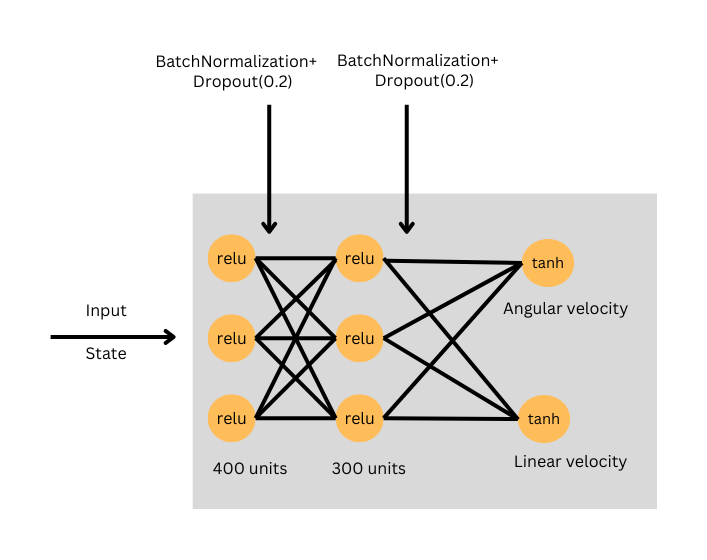
\includegraphics[scale=0.60]{actor_net}
\caption[actor network]{actor network}
\end{figure}

 \begin{figure}[h]  
\centering
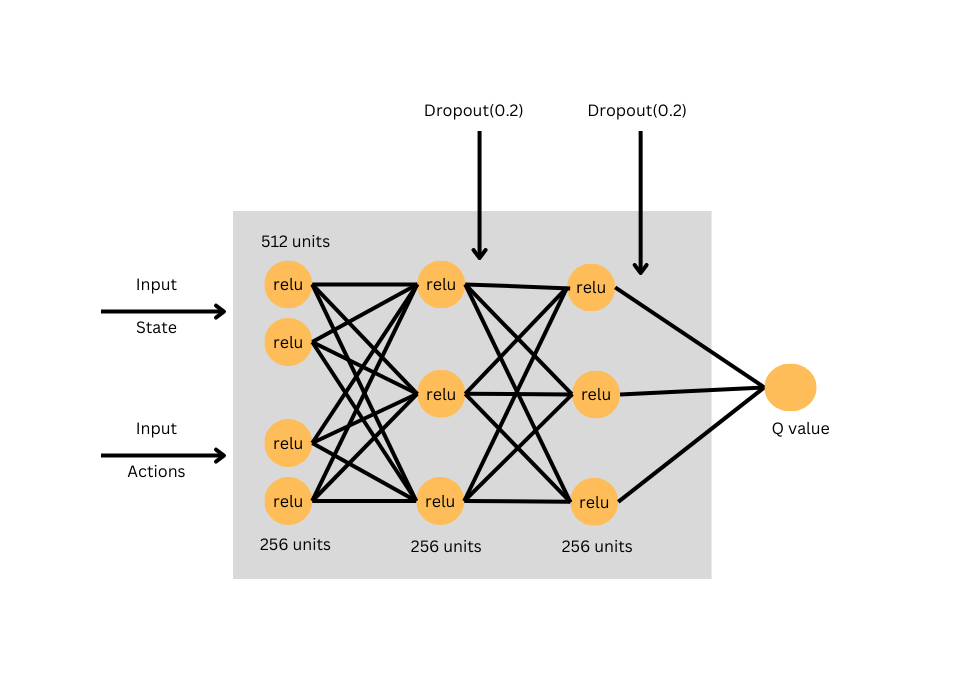
\includegraphics[scale=0.60]{critic_net}
\caption[critic network]{critic network}
\end{figure}

\afterpage{\clearpage}








\newpage
\pagebreak
\hspace{0pt}
\vfill
\begin{center}
\section{Result and analysis}
\end{center}
\vfill
\hspace{0pt}

\pagebreak

\subsection{Introdution}

In this last section, we will describe the results that we get from our experiment and discuss them.



\begin{figure}[h]  

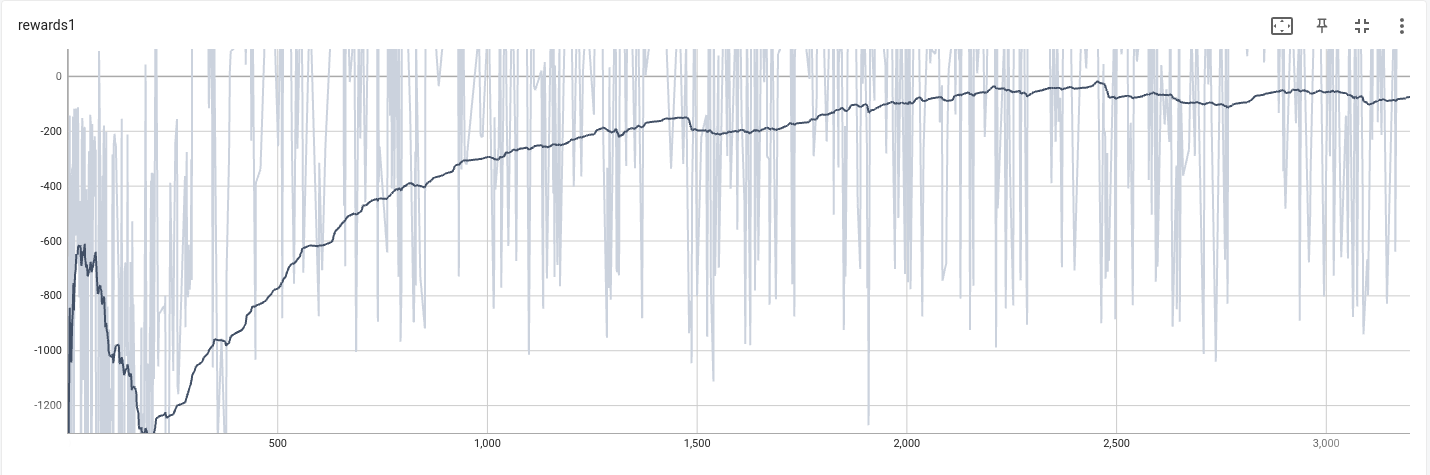
\includegraphics[scale=0.40]{robot1}
\caption[robot1]{robot1}
\end{figure}

\begin{figure}[h]  

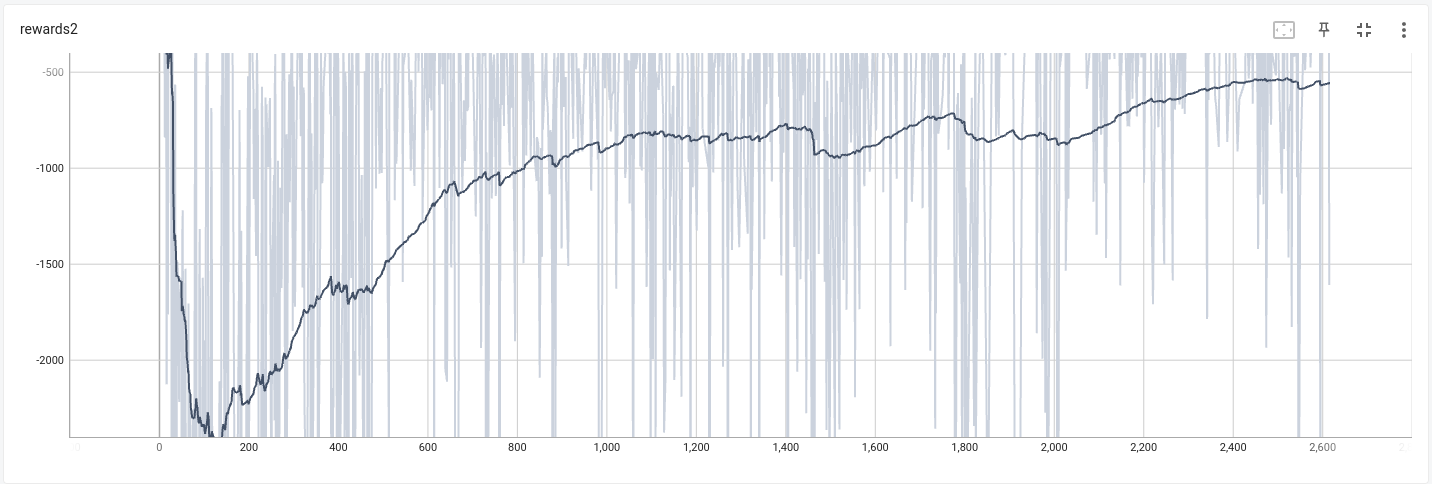
\includegraphics[scale=0.40]{robot2}
\caption[robot2]{robot2}
\end{figure}

\begin{figure}[h]  

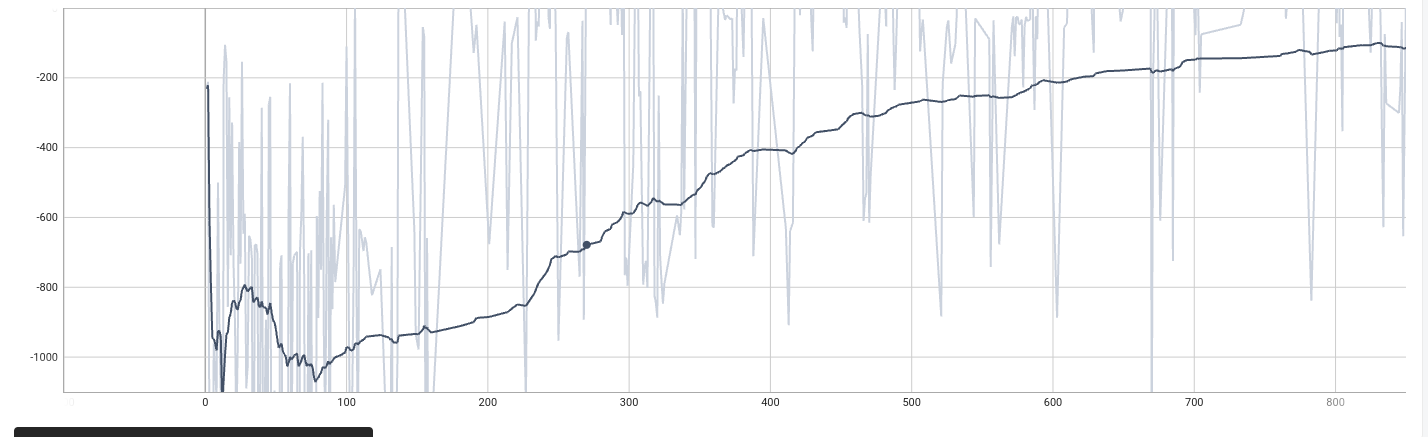
\includegraphics[scale=0.40]{robot3}
\caption[robot3]{robot3}
\end{figure}

\begin{figure}[h]  

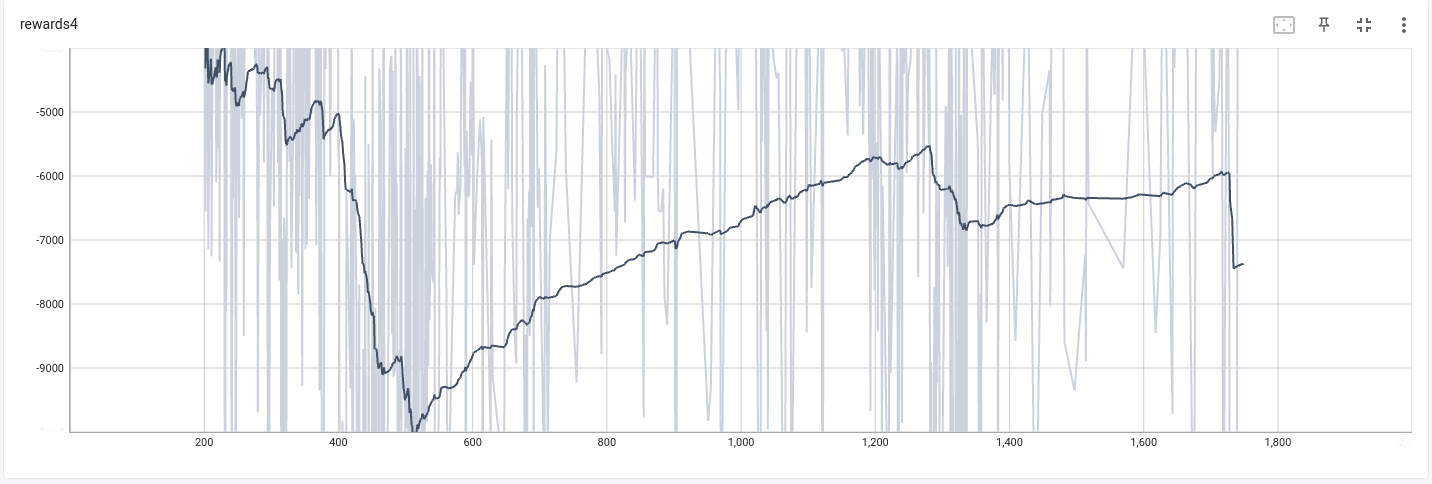
\includegraphics[scale=0.40]{robot4}
\caption[robot4]{robot4}
\end{figure}

 


\newpage
\bibliography{bib}
\bibliographystyle{ieeetr}



\end{document}
